\subsubsection{Свеска 10}

\zadatak
Реши неједначину
$$
\log_5 x \ge \frac12 \log_5(3x-2).
$$

\resenje
Да би логаритам био дефинисан, видимо да мора бити
$$
3x-2>0\sledi x>\frac23.
$$
Ако неједначину поможимо са 2, добијамо
\begin{align*}
    2\log_5 x   &\ge \log_5(3x-2)\\
    \log_5 x^2  &\ge \log_5(3x-2)\\
    x^2 &\ge 3x-2\\
    x^2 -3x + 2 &\ge 0.
\end{align*}
Квадратна једначина\queq\ има решења $x_1=1$ и $x_2=2$,
па је решење неједначине
$$
x\in\ram{\left( \frac23, 1 \right] \cup  [2, \infty )}.
$$
$$
\slika{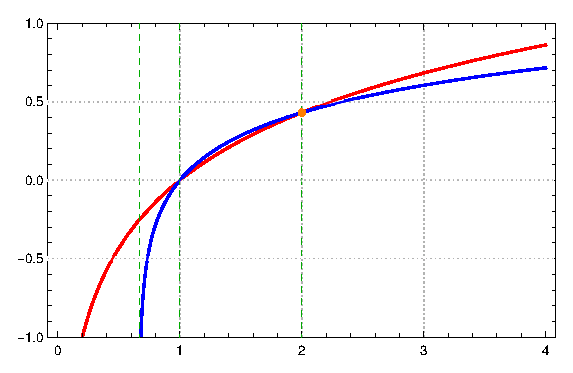
\includegraphics[width=\sirina]{eps/10.eps}}{$y={\color{red}\log_5 x};\, {\color{blue}\frac12 \log_5(3x-2)}$.}
$$

